\chapter{Dynaaminen ohjelmointi}

\index{dynaaminen ohjelmointi@dynaaminen ohjelmointi}

\key{Dynaaminen ohjelmointi}
on tekniikka, joka yhdistää täydellisen haun
toimivuuden ja ahneiden algoritmien tehokkuuden.
Dynaamisen ohjelmoinnin käyttäminen edellyttää,
että tehtävä jakautuu osaongelmiin,
jotka voidaan käsitellä toisistaan riippumattomasti.

Dynaamisella ohjelmoinnilla on kaksi käyttötarkoitusta:

\begin{itemize}
\item
\key{Optimiratkaisun etsiminen}:
Haluamme etsiä ratkaisun, joka on
jollakin tavalla suurin mahdollinen
tai pienin mahdollinen.
\item
\key{Ratkaisuiden määrän laskeminen}:
Haluamme laskea, kuinka monta mahdollista
ratkaisua on olemassa.
\end{itemize}

Tutustumme dynaamiseen ohjelmointiin ensin
optimiratkaisun etsimisen kautta ja käytämme sitten
samaa ideaa ratkaisujen määrän laskemiseen.

Dynaamisen ohjelmoinnin ymmärtäminen on yksi merkkipaalu
jokaisen kisakoodarin uralla.
Vaikka menetelmän perusidea on yksinkertainen,
haasteena on oppia soveltamaan sitä sujuvasti
erilaisissa tehtävissä.
Tämä luku esittelee joukon
perusesimerkkejä, joista on hyvä lähteä liikkeelle.

\section{Kolikkotehtävä}

Aloitamme dynaamisen ohjelmoinnin tutun tehtävän kautta:

\begin{task}
Kolikoiden arvot ovat $\{c_1,c_2,\ldots,c_k\}$,
ja tehtäväsi on muodostaa kolikoista rahamäärä $x$.
Jokaista kolikkoa on saatavilla rajattomasti.
Mikä on pienin määrä kolikoita,
joilla rahamäärän voi muodostaa?
\end{task}

Luvussa 6.1 ratkaisimme tehtävän ahneella algoritmilla,
joka muodostaa rahamäärän valiten mahdollisimman
suuria kolikoita.
Ahne algoritmi toimii esimerkiksi silloin,
kun kolikot ovat eurokolikot,
mutta yleisessä tapauksessa ahne algoritmi
ei välttämättä valitse pienintä määrää kolikoita.

Nyt on aika ratkaista tehtävä tehokkaasti
dynaamisella ohjelmoinnilla niin,
että algoritmi toimii millä tahansa kolikoilla.

\subsubsection{Rekursiivinen esitys}

\index{rekursioyhtxlz@rekursioyhtälö}

Dynaamisessa ohjelmoinnissa on ideana esittää
ongelma rekursiivisesti niin,
että ongelman ratkaisun voi laskea
saman ongelman pienempien tapausten ratkaisuista.
Tässä tehtävässä luonteva ongelma on seuraava:
mikä on pienin määrä kolikoita,
joilla voi muodostaa rahamäärän $x$?

Merkitään $f(x)$ funktiota,
joka antaa vastauksen ongelmaan,
eli $f(x)$ on pienin määrä kolikoita,
joilla voi muodostaa rahamäärän $x$.
Funktion arvot riippuvat siitä,
mitkä kolikot ovat käytössä.
Esimerkiksi jos kolikot ovat $\{1,3,4\}$,
funktion ensimmäiset arvot ovat:

\[
\begin{array}{lcl}
f(0) & = & 0 \\
f(1) & = & 1 \\
f(2) & = & 2 \\
f(3) & = & 1 \\
f(4) & = & 1 \\
f(5) & = & 2 \\
f(6) & = & 2 \\
f(7) & = & 2 \\
f(8) & = & 2 \\
f(9) & = & 3 \\
f(10) & = & 3 \\
\end{array}
\]

Nyt $f(0)=0$, koska jos rahamäärä on 0,
ei tarvita yhtään kolikkoa.
Vastaavasti $f(3)=1$, koska rahamäärän 3
voi muodostaa kolikolla 3,
ja $f(5)=2$, koska rahamäärän 5
voi muodostaa kolikoilla 1 ja 4.

Oleellinen ominaisuus funktiossa on,
että arvon $f(x)$ pystyy laskemaan
rekursiivisesti käyttäen pienempiä
funktion arvoja.
Esimerkiksi jos kolikot ovat $\{1,3,4\}$,
on kolme tapaa alkaa muodostaa rahamäärää $x$:
valitaan kolikko 1, 3 tai 4.
Jos valitaan kolikko 1, täytyy
muodostaa vielä rahamäärä $x-1$.
Vastaavasti jos valitaan kolikko 3 tai 4,
täytyy muodostaa rahamäärä $x-3$ tai $x-4$.

Niinpä rekursiivinen kaava on
\[f(x) = \min(f(x-1),f(x-3),f(x-4))+1,\]
missä funktio $\min$ valitsee pienimmän parametreistaan.
Yleisemmin jos kolikot ovat $\{c_1,c_2,\ldots,c_k\}$,
rekursiivinen kaava on
\[f(x) = \min(f(x-c_1),f(x-c_2),\ldots,f(x-c_k))+1.\]
Funktion pohjatapauksena on
\[f(0)=0,\]
koska rahamäärän 0 muodostamiseen ei tarvita
yhtään kolikkoa.
Lisäksi on hyvä määritellä
\[f(x)=\infty,\hspace{8px}\textrm{jos $x<0$}.\]
Tämä tarkoittaa, että negatiivisen rahamäärän
muodostaminen vaatii äärettömästi kolikoita,
mikä estää sen, että rekursio muodostaisi
ratkaisun, johon kuuluu negatiivinen rahamäärä.

Nyt voimme toteuttaa funktion C++:lla suoraan
rekursiivisen määritelmän perusteella:

\begin{lstlisting}
int f(int x) {
    if (x == 0) return 0;
    if (x < 0) return 1e9;
    int u = 1e9;
    for (int i = 1; i <= k; i++) {
        u = min(u, f(x-c[i])+1);
    }
    return u;
}
\end{lstlisting}

Koodi olettaa, että käytettävät kolikot ovat
$\texttt{c}[1], \texttt{c}[2], \ldots, \texttt{c}[n]$,
ja arvo $10^9$ kuvastaa ääretöntä.
Tämä on toimiva funktio, mutta se ei ole vielä tehokas,
koska funktio käy läpi valtavasti erilaisia tapoja
muodostaa rahamäärä.
Seuraavaksi esiteltävä muistitaulukko tekee
funktiosta tehokkaan.

\subsubsection{Muistitaulukko}

\index{muistitaulukko@muistitaulukko}

Dynaaminen ohjelmointi tehostaa
rekursiivisen funktion laskentaa
tallentamalla funktion arvoja \key{muistitaulukkoon}.
Taulukon avulla funktion arvo
tietyllä parametrilla riittää laskea
vain kerran, minkä jälkeen sen voi
hakea suoraan taulukosta.
Tämä muutos nopeuttaa algoritmia ratkaisevasti.

Tässä tehtävässä muistitaulukoksi sopii taulukko

\begin{lstlisting}
int d[N];
\end{lstlisting}

jonka kohtaan $\texttt{d}[x]$
lasketaan funktion arvo $f(x)$.
Vakio $N$ valitaan niin, että kaikki
laskettavat funktion arvot mahtuvat taulukkoon.

Tämän jälkeen funktion voi toteuttaa
tehokkaasti näin:

\begin{lstlisting}
int f(int x) {
    if (x == 0) return 0;
    if (x < 0) return 1e9;
    if (d[x]) return d[x];
    int u = 1e9;
    for (int i = 1; i <= k; i++) {
        u = min(u, f(x-c[i])+1);
    }
    d[x] = u;
    return d[x];
}
\end{lstlisting}

Funktio käsittelee pohjatapaukset $x=0$
ja $x<0$ kuten ennenkin.
Sitten funktio tarkastaa,
onko $f(x)$ laskettu jo taulukkoon $\texttt{d}[x]$.
Jos $f(x)$ on laskettu,
funktio palauttaa sen suoraan.
Muussa tapauksessa funktio laskee arvon rekursiivisesti
ja tallentaa sen kohtaan $\texttt{d}[x]$.

Muistitaulukon ansiosta funktio toimii
nopeasti, koska sen tarvitsee laskea
vastaus kullekin $x$:n arvolle
vain kerran rekursiivisesti.
Heti kun arvo $f(x)$ on tallennettu muistitaulukkoon,
sen saa haettua sieltä suoraan,
kun funktiota kutsutaan seuraavan kerran parametrilla $x$.

Tuloksena olevan algoritmin aikavaativuus on $O(xk)$,
kun rahamäärä on $x$ ja kolikoiden määrä on $k$.
Käytännössä ratkaisu on mahdollista toteuttaa,
jos $x$ on niin pieni, että on mahdollista varata 
riittävän suuri muistitaulukko.

Huomaa, että muistitaulukon voi muodostaa
myös suoraan silmukalla ilman rekursiota
laskemalla arvot pienimmästä suurimpaan:
\begin{lstlisting}
d[0] = 0;
for (int i = 1; i <= x; i++) {
    int u = 1e9;
    for (int j = 1; j <= k; j++) {
        if (i-c[j] < 0) continue;
        u = min(u, d[i-c[j]]+1);
    }
    d[i] = u;
}
\end{lstlisting}

Silmukkatoteutus on lyhyempi ja
hieman tehokkaampi kuin rekursiototeutus,
minkä vuoksi kokeneet kisakoodarit
toteuttavat dynaamisen ohjelmoinnin
usein silmukan avulla.
Kuitenkin silmukkatoteutuksen taustalla
on sama rekursiivinen idea kuin ennenkin.

\subsubsection{Ratkaisun muodostaminen}

Joskus optimiratkaisun arvon selvittämisen lisäksi
täytyy muodostaa näytteeksi yksi mahdollinen optimiratkaisu.
Tässä tehtävässä tämä tarkoittaa,
että ohjelman täytyy antaa esimerkki
tavasta valita kolikot,
joista muodostuu rahamäärä $x$
käyttäen mahdollisimman vähän kolikoita.

Ratkaisun muodostaminen onnistuu lisäämällä
koodiin uuden taulukon, joka kertoo
kullekin rahamäärälle,
mikä kolikko siitä tulee poistaa
optimiratkaisussa.
Seuraavassa koodissa taulukko \texttt{e}
huolehtii asiasta:

\begin{lstlisting}
d[0] = 0;
for (int i = 1; i <= x; i++) {
    d[i] = 1e9;
    for (int j = 1; j <= k; j++) {
        if (i-c[j] < 0) continue;
        int u = d[i-c[j]]+1;
        if (u < d[i]) {
            d[i] = u;
            e[i] = c[j];
        }
    }
}
\end{lstlisting}

Tämän jälkeen rahamäärän $x$ muodostavat
kolikot voi tulostaa näin:

\begin{lstlisting}
while (x > 0) {
    cout << e[x] << "\n";
    x -= e[x];
}
\end{lstlisting}

\subsubsection{Ratkaisuiden määrän laskeminen}

Tarkastellaan sitten tehtävän muunnelmaa,
jossa laskettavana on ratkaisuiden yhteismäärä:
\begin{task}
Kolikoiden arvot ovat $\{c_1,c_2,\ldots,c_k\}$,
ja tehtäväsi on muodostaa kolikoista rahamäärä $x$.
Jokaista kolikkoa on saatavilla rajattomasti.
Monellako eri tavalla voit muodostaa rahamäärän?
\end{task}

\noindent
Esimerkiksi jos kolikot ovat $\{1,3,4\}$ ja rahamäärä on 5,
niin ratkaisuja on 6:

%\begin{multicols}{2}
\begin{itemize}[noitemsep]
\item $1+1+1+1+1$
\item $1+1+3$
\item $1+3+1$
\item $3+1+1$
\item $1+4$
\item $4+1$
\end{itemize}
%\end{multicols}

Ratkaisujen määrän laskeminen tapahtuu melko samalla tavalla
kuin optimiratkaisun etsiminen.
Erona on, että optimiratkaisun etsivässä rekursiossa
valitaan yleensä pienin tai suurin aiempi arvo,
kun taas ratkaisujen määrän laskevassa rekursiossa lasketaan
yhteen kaikki vaihtoehdot.

Tässä tapauksessa voimme muodostaa funktion $f(x)$,
joka kertoo, monellako tavalla rahamäärän $x$
voi muodostaa kolikoista.
Esimerkiksi $f(5)=6$, kun kolikot ovat $\{1,3,4\}$.

Funktion $f(x)$ saa laskettua rekursiivisesti kaavalla

\[ f(x) = f(x-c_1)+f(x-c_2)+\cdots+f(x-c_k),\]

\noindent
koska rahamäärän $x$ muodostamiseksi pitää
valita jokin kolikko $c_i$ ja muodostaa sen jälkeen rahamäärä $x-c_i$.
Pohjatapauksina ovat $f(0)=1$, koska rahamäärä 0 syntyy
ilman yhtään kolikkoa,
sekä $f(x)=0$, kun $x<0$, koska negatiivista rahamäärää
ei ole mahdollista muodostaa.

Yllä olevassa esimerkissä funktioksi tulee

\[ f(x) = f(x-1)+f(x-3)+f(x-4), \]

ja funktion ensimmäiset arvot ovat:

\[
\begin{array}{lcl}
f(0) & = & 1 \\
f(1) & = & 1 \\
f(2) & = & 1 \\
f(3) & = & 2 \\
f(4) & = & 4 \\
f(5) & = & 6 \\
f(6) & = & 9 \\
f(7) & = & 15 \\
f(8) & = & 25 \\
f(9) & = & 40 \\
\end{array}
\]

Seuraava koodi laskee funktion $f(x)$ arvon
dynaamisella ohjelmoinnilla täyttämällä taulukon
\texttt{d} rahamäärille $0 \ldots x$:

\begin{lstlisting}
d[0] = 1;
for (int i = 1; i <= x; i++) {
    for (int j = 1; j <= k; j++) {
        if (i-c[j] < 0) continue;
        d[i] += d[i-c[j]];
    }
}
\end{lstlisting}

Usein ratkaisujen määrä on niin suuri, että sitä ei tarvitse
laskea kokonaan vaan riittää ilmoittaa vastaus
modulo $m$, missä esimerkiksi $m=10^9+7$.
Tämä onnistuu muokkaamalla koodia niin,
että kaikki laskutoimitukset lasketaan modulo $m$.
Tässä tapauksessa riittää lisätä rivin
\begin{lstlisting}
        d[i] += d[i-c[j]];
\end{lstlisting}
jälkeen rivi
\begin{lstlisting}
        d[i] %= m;
\end{lstlisting}

\section{Pisin nouseva alijono}

\index{pisin nouseva alijono@pisin nouseva alijono}

\begin{task}
Taulukossa on $n$ kokonaislukua $x_1,x_2,\ldots,x_n$.
Tehtäväsi on selvittää taulukon
\key{pisin nouseva alijono}, joka muodostuu
joukosta taulukon lukuja niin, että kukin
luku on edellistä suurempi.
\end{task}

\begin{samepage}
Esimerkiksi taulukossa

\begin{center}
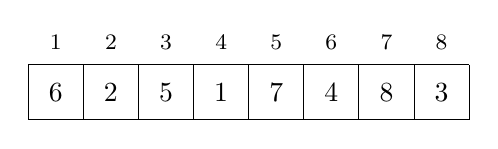
\begin{tikzpicture}[scale=0.7]
\draw (0,0) grid (8,1);
\node at (0.5,0.5) {$6$};
\node at (1.5,0.5) {$2$};
\node at (2.5,0.5) {$5$};
\node at (3.5,0.5) {$1$};
\node at (4.5,0.5) {$7$};
\node at (5.5,0.5) {$4$};
\node at (6.5,0.5) {$8$};
\node at (7.5,0.5) {$3$};

\footnotesize
\node at (0.5,1.4) {$1$};
\node at (1.5,1.4) {$2$};
\node at (2.5,1.4) {$3$};
\node at (3.5,1.4) {$4$};
\node at (4.5,1.4) {$5$};
\node at (5.5,1.4) {$6$};
\node at (6.5,1.4) {$7$};
\node at (7.5,1.4) {$8$};
\end{tikzpicture}
\end{center}
\end{samepage}
pisin nouseva alijono sisältää 4 lukua:
\begin{center}
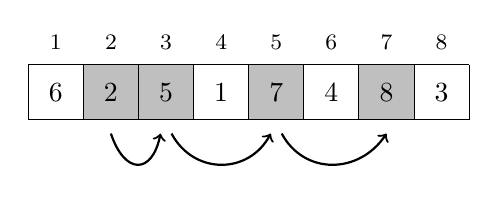
\begin{tikzpicture}[scale=0.7]
\fill[color=lightgray] (1,0) rectangle (2,1);
\fill[color=lightgray] (2,0) rectangle (3,1);
\fill[color=lightgray] (4,0) rectangle (5,1);
\fill[color=lightgray] (6,0) rectangle (7,1);
\draw (0,0) grid (8,1);
\node at (0.5,0.5) {$6$};
\node at (1.5,0.5) {$2$};
\node at (2.5,0.5) {$5$};
\node at (3.5,0.5) {$1$};
\node at (4.5,0.5) {$7$};
\node at (5.5,0.5) {$4$};
\node at (6.5,0.5) {$8$};
\node at (7.5,0.5) {$3$};

\draw[thick,->] (1.5,-0.25) .. controls (1.75,-1.00) and (2.25,-1.00) .. (2.4,-0.25);
\draw[thick,->] (2.6,-0.25) .. controls (3.0,-1.00) and (4.0,-1.00) .. (4.4,-0.25);
\draw[thick,->] (4.6,-0.25) .. controls (5.0,-1.00) and (6.0,-1.00) .. (6.5,-0.25);

\footnotesize
\node at (0.5,1.4) {$1$};
\node at (1.5,1.4) {$2$};
\node at (2.5,1.4) {$3$};
\node at (3.5,1.4) {$4$};
\node at (4.5,1.4) {$5$};
\node at (5.5,1.4) {$6$};
\node at (6.5,1.4) {$7$};
\node at (7.5,1.4) {$8$};
\end{tikzpicture}
\end{center}

Merkitään $f(k)$ kohtaan $k$ päättyvän
pisimmän nousevan alijonon pituutta,
jolloin ratkaisu tehtävään on suurin
arvoista $f(1),f(2),\ldots,f(n)$.
Esimerkiksi yllä olevassa taulukossa
funktion arvot ovat seuraavat:
\[
\begin{array}{lcl}
f(1) & = & 1 \\
f(2) & = & 1 \\
f(3) & = & 2 \\
f(4) & = & 1 \\
f(5) & = & 3 \\
f(6) & = & 2 \\
f(7) & = & 4 \\
f(8) & = & 2 \\
\end{array}
\]

Arvon $f(k)$ laskemisessa on kaksi vaihtoehtoa,
millainen kohtaan $k$ päättyvä pisin nouseva alijono on:
\begin{enumerate}
\item Pisin nouseva alijono sisältää vain luvun $x_k$,
jolloin $f(k)=1$.
\item Valitaan jokin kohta $i$, jolle pätee $i<k$
ja $x_i<x_k$.
Pisin nouseva alijono saadaan liittämällä
kohtaan $i$ päättyvän pisimmän nousevan alijonon perään luku $x_k$.
Tällöin $f(k)=f(i)+1$.
\end{enumerate}

Tarkastellaan esimerkkinä arvon $f(7)$ laskemista.
Paras ratkaisu on ottaa pohjaksi kohtaan 5
päättyvä pisin nouseva alijono $[2,5,7]$
ja lisätä sen perään luku $x_7=8$.
Tuloksena on alijono $[2,5,7,8]$ ja $f(7)=f(5)+1=4$.

Suoraviivainen tapa toteuttaa algoritmi on
käydä kussakin kohdassa $k$ läpi kaikki kohdat
$i=1,2,\ldots,k-1$, joissa voi olla alijonon
edellinen luku.
Tällaisen algoritmin aikavaativuus on $O(n^2)$.
Yllättävää kyllä, algoritmin voi toteuttaa myös
ajassa $O(n \log n)$, mutta tämä on vaikeampaa.

\section{Reitinhaku ruudukossa}

\begin{task}
Tehtäväsi on etsiä $n \times n$ -ruudukossa
reitti vasemmasta yläkulmasta oikeaan alakulmaan
niin, että lukujen summa reitillä on mahdollisimman suuri.
Saat liikkua joka askeleella yhden ruudun
oikealle tai alaspäin.
\end{task}

Seuraavassa ruudukossa paras reitti
on merkitty harmaalla taustalla:
\begin{center}
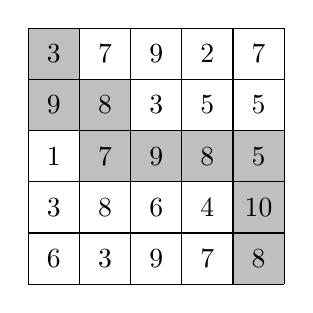
\begin{tikzpicture}[scale=.65]
  \begin{scope}
    \fill [color=lightgray] (0, 9) rectangle (1, 8);
    \fill [color=lightgray] (0, 8) rectangle (1, 7);
    \fill [color=lightgray] (1, 8) rectangle (2, 7);
    \fill [color=lightgray] (1, 7) rectangle (2, 6);
    \fill [color=lightgray] (2, 7) rectangle (3, 6);
    \fill [color=lightgray] (3, 7) rectangle (4, 6);
    \fill [color=lightgray] (4, 7) rectangle (5, 6);
    \fill [color=lightgray] (4, 6) rectangle (5, 5);
    \fill [color=lightgray] (4, 5) rectangle (5, 4);
    \draw (0, 4) grid (5, 9);
    \node at (0.5,8.5) {3};
    \node at (1.5,8.5) {7};
    \node at (2.5,8.5) {9};
    \node at (3.5,8.5) {2};
    \node at (4.5,8.5) {7};
    \node at (0.5,7.5) {9};
    \node at (1.5,7.5) {8};
    \node at (2.5,7.5) {3};
    \node at (3.5,7.5) {5};
    \node at (4.5,7.5) {5};
    \node at (0.5,6.5) {1};
    \node at (1.5,6.5) {7};
    \node at (2.5,6.5) {9};
    \node at (3.5,6.5) {8};
    \node at (4.5,6.5) {5};
    \node at (0.5,5.5) {3};
    \node at (1.5,5.5) {8};
    \node at (2.5,5.5) {6};
    \node at (3.5,5.5) {4};
    \node at (4.5,5.5) {10};
    \node at (0.5,4.5) {6};
    \node at (1.5,4.5) {3};
    \node at (2.5,4.5) {9};
    \node at (3.5,4.5) {7};
    \node at (4.5,4.5) {8};
  \end{scope}
\end{tikzpicture}
\end{center}

Tällä reitillä lukujen summa on $3+9+8+7+9+8+5+10+8=67$,
joka on suurin mahdollinen summa vasemmasta yläkulmasta
oikeaan alakulmaan.

Hyvä lähestymistapa tehtävään on laskea
kuhunkin ruutuun $(y,x)$ suurin summa
reitillä vasemmasta yläkulmasta kyseiseen ruutuun.
Merkitään tätä suurinta summaa $f(y,x)$,
jolloin $f(n,n)$ on suurin summa
reitillä vasemmasta yläkulmasta oikeaan alakulmaan.

Rekursio syntyy havainnosta,
että ruutuun $(y,x)$ saapuvan reitin
täytyy tulla joko vasemmalta ruudusta $(y,x-1)$
tai ylhäältä ruudusta $(y-1,x)$:
\begin{center}
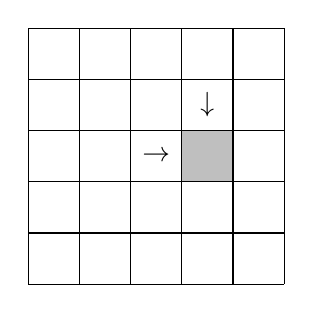
\begin{tikzpicture}[scale=.65]
  \begin{scope}
    \fill [color=lightgray] (3, 7) rectangle (4, 6);
    \draw (0, 4) grid (5, 9);
    
    \node at (2.5,6.5) {$\rightarrow$};
    \node at (3.5,7.5) {$\downarrow$};
    
  \end{scope}
\end{tikzpicture}
\end{center}

Kun $r(y,x)$
on ruudukon luku kohdassa $(y,x)$,
rekursion pohjatapaukset ovat seuraavat:

\[
\begin{array}{lcl}
f(1,1) & = & r(1,1) \\
f(1,x) & = & f(1,x-1)+r(1,x) \\
f(y,1) & = & f(y-1,1)+r(y,1)\\
\end{array}
\]

Yleisessä tapauksessa valittavana on
kaksi reittiä,
joista kannattaa valita se,
joka tuottaa suuremman summan:
\[ f(y,x) = \max(f(y,x-1),f(y-1,x))+r(y,x)\]

Ratkaisun aikavaativuus on $O(n^2)$, koska jokaisessa
ruudussa $f(y,x)$ saadaan laskettua vakioajassa
viereisten ruutujen arvoista.

\section{Repunpakkaus}

\index{repunpakkaus@repunpakkaus}

\begin{task}
Sinulla on $n$ tavaraa, joiden painot ovat
$p_1,p_2,\ldots,p_n$ ja arvot ovat
$a_1,a_2,\ldots,a_n$.
Tehtäväsi on valita reppuun pakattavat tavarat
niin, että painojen summa on enintään $x$
ja arvojen summa on mahdollisimman suuri.
\end{task}

\begin{samepage}
Esimerkiksi jos tavarat ovat
\begin{center}
\begin{tabular}{rrr}
tavara & paino & arvo \\
\hline
A & 5 & 1 \\
B & 6 & 3 \\
C & 8 & 5 \\
D & 5 & 3 \\
\end{tabular}
\end{center}
\end{samepage}
ja suurin sallittu yhteispaino on 12,
niin paras ratkaisu on pakata reppuun tavarat $B$ ja $D$.
Niiden yhteispaino $6+5=11$ ei ylitä rajaa 12
ja arvojen summa
on $3+3=6$, mikä on paras mahdollinen tulos.

Tämä tehtävä on mahdollista ratkaista kahdella eri
tavalla dynaamisella ohjelmoinnilla
riippuen siitä, tarkastellaanko ongelmaa
maksimointina vai minimointina.
Käymme seuraavaksi läpi molemmat ratkaisut.

\subsubsection{Ratkaisu 1}

\textit{Maksimointi:} Merkitään $f(k,u)$
suurinta mahdollista tavaroiden yhteisarvoa,
kun reppuun pakataan jokin osajoukko
tavaroista $1 \ldots k$,
jossa tavaroiden yhteispaino on $u$.
Ratkaisu tehtävään on suurin arvo
$f(n,u)$, kun $0 \le u \le x$.
Rekursiivinen kaava funktion laskemiseksi on
\[f(k,u) = \max(f(k-1,u),f(k-1,u-p_k)+a_k),\]
koska kohdassa $k$ oleva tavara joko otetaan tai ei oteta
mukaan ratkaisuun.
Pohjatapauksina on $f(0,0)=0$ ja $f(0,u)=-\infty$,
kun $u \neq 0$. Tämän ratkaisun aikavaativuus on $O(nx)$.

\subsubsection{Ratkaisu 2}

\textit{Minimointi:} Merkitään $f(k,u)$
pienintä mahdollista tavaroiden yhteispainoa,
kun reppuun pakataan jokin osajoukko
tavaroista $1 \ldots k$,
jossa tavaroiden yhteisarvo on $u$.
Ratkaisu tehtävään on suurin arvo $u$,
jolle pätee $0 \le u \le s$ ja $f(n,u) \le x$,
missä $s=\sum_{i=1}^n a_i$.
Rekursiivinen kaava funktion laskemiseksi on
\[f(k,u) = \min(f(k-1,u),f(k-1,u-a_k)+p_k)\]
ratkaisua 1 vastaavasti.
Pohjatapauksina on $f(0,0)=0$ ja $f(0,u)=\infty$, kun $u \neq 0$.
Tämän ratkaisun aikavaativuus on $O(ns)$.

~\\
Kiinnostava seikka on, että eri asiat syötteessä
vaikuttavat ratkaisuiden tehokkuuteen.
Ratkaisussa 1 tavaroiden painot vaikuttavat tehokkuuteen
mutta arvoilla ei ole merkitystä.
Ratkaisussa 2 puolestaan tavaroiden arvot vaikuttavat
tehokkuuteen mutta painoilla ei ole merkitystä.

\section{Editointietäisyys}

\index{editointietxisyys@editointietäisyys}
\index{Levenšteinin etäisyys}

\key{Editointietäisyys} eli
\key{Levenšteinin etäisyys}
kuvaa, kuinka kaukana kaksi merkkijonoa ovat toisistaan.
Se on pienin määrä editointioperaatioita,
joilla ensimmäisen merkkijonon saa muutettua toiseksi.
Sallitut operaatiot ovat:
\begin{itemize}
\item merkin lisäys (esim. \texttt{ABC} $\rightarrow$ \texttt{ABCA})
\item merkin poisto (esim. \texttt{ABC} $\rightarrow$ \texttt{AC})
\item merkin muutos (esim. \texttt{ABC} $\rightarrow$ \texttt{ADC})
\end{itemize}

Esimerkiksi merkkijonojen \texttt{TALO} ja \texttt{PALLO}
editointietäisyys on 2, koska voi tehdä ensin
operaation \texttt{TALO} $\rightarrow$ \texttt{TALLO}
(merkin lisäys) ja sen jälkeen operaation
\texttt{TALLO} $\rightarrow$ \texttt{PALLO}
(merkin muutos).
Tämä on pienin mahdollinen määrä operaatioita, koska
selvästikään yksi operaatio ei riitä.

Tutustumme editointietäisyyteen seuraavan tehtävän kautta:
\begin{task}
Annettuna on merkkijono \texttt{x},
jossa on $n$ merkkiä,
sekä merkkijono \texttt{y},
jossa on $m$ merkkiä.
Mikä on merkkijonojen editointietäisyys ja
miten editoinnin voi suorittaa?
\end{task}

Merkkijonojen \texttt{x} ja \texttt{y}
editointietäisyyden voi
laskea dynaamisella ohjelmoinnilla ajassa $O(nm)$.
Merkitään funktiolla $f(a,b)$
editointietäisyyttä \texttt{x}:n $a$
ensimmäisen merkin sekä
\texttt{y}:n $b$:n ensimmäisen merkin välillä.
Tämän funktion avulla saa sekä
laskettua tehokkaasti editointietäisyyden että
selvitettyä, mitkä ovat tarvittavat editointioperaatiot.
Funktion pohjatapaukset ovat
\[
\begin{array}{lcl}
f(0,b) & = & b \\
f(a,0) & = & a \\
\end{array}
\]
ja yleisessä tapauksessa pätee kaava
\[ f(a,b) = \min(f(a,b-1)+1,f(a-1,b)+1,f(a-1,b-1)+c),\]
missä $c=0$, jos \texttt{x}:n merkki $a$
ja \texttt{y}:n merkki $b$ ovat samat,
ja muussa tapauksessa $c=1$.
Kaava käy läpi mahdollisuudet lyhentää merkkijonoja:
\begin{itemize}
\item $f(a,b-1)$ tarkoittaa, että $x$:ään lisätään merkki
\item $f(a-1,b)$ tarkoittaa, että $x$:stä poistetaan merkki
\item $f(a-1,b-1)$ tarkoittaa, että $x$:ssä ja $y$:ssä on
sama merkki ($c=0$) tai $x$:n merkki muutetaan $y$:n merkiksi ($c=1$)
\end{itemize}

Seuraava taulukko sisältää funktion $f$ arvot
esimerkin tapauksessa:
\begin{center}
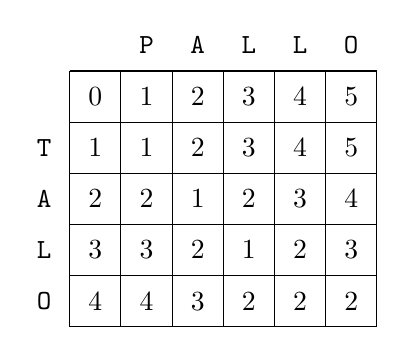
\begin{tikzpicture}[scale=.65]
  \begin{scope}
    %\fill [color=lightgray] (5, -3) rectangle (6, -4);
    \draw (1, -1) grid (7, -6);
    
    \node at (0.5,-2.5) {\texttt{T}};
    \node at (0.5,-3.5) {\texttt{A}};
    \node at (0.5,-4.5) {\texttt{L}};
    \node at (0.5,-5.5) {\texttt{O}};

    \node at (2.5,-0.5) {\texttt{P}};
    \node at (3.5,-0.5) {\texttt{A}};
    \node at (4.5,-0.5) {\texttt{L}};
    \node at (5.5,-0.5) {\texttt{L}};
    \node at (6.5,-0.5) {\texttt{O}};

    \node at (1.5,-1.5) {$0$};
    \node at (1.5,-2.5) {$1$};
    \node at (1.5,-3.5) {$2$};
    \node at (1.5,-4.5) {$3$};
    \node at (1.5,-5.5) {$4$};
    \node at (2.5,-1.5) {$1$};
    \node at (2.5,-2.5) {$1$};
    \node at (2.5,-3.5) {$2$};
    \node at (2.5,-4.5) {$3$};
    \node at (2.5,-5.5) {$4$};
    \node at (3.5,-1.5) {$2$};
    \node at (3.5,-2.5) {$2$};
    \node at (3.5,-3.5) {$1$};
    \node at (3.5,-4.5) {$2$};
    \node at (3.5,-5.5) {$3$};
    \node at (4.5,-1.5) {$3$};
    \node at (4.5,-2.5) {$3$};
    \node at (4.5,-3.5) {$2$};
    \node at (4.5,-4.5) {$1$};
    \node at (4.5,-5.5) {$2$};
    \node at (5.5,-1.5) {$4$};
    \node at (5.5,-2.5) {$4$};
    \node at (5.5,-3.5) {$3$};
    \node at (5.5,-4.5) {$2$};
    \node at (5.5,-5.5) {$2$};
    \node at (6.5,-1.5) {$5$};
    \node at (6.5,-2.5) {$5$};
    \node at (6.5,-3.5) {$4$};
    \node at (6.5,-4.5) {$3$};
    \node at (6.5,-5.5) {$2$};
  \end{scope}
\end{tikzpicture}
\end{center}

Taulukon oikean alanurkan ruutu
kertoo, että merkkijonojen \texttt{TALO}
ja \texttt{PALLO} editointietäisyys on 2.
Taulukosta pystyy myös
lukemaan, miten pienimmän editointietäisyyden
voi saavuttaa.
Tässä tapauksessa polku on seuraava:

\begin{center}
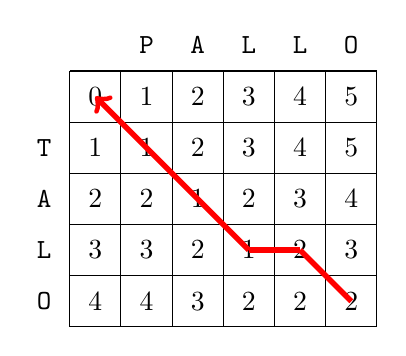
\begin{tikzpicture}[scale=.65]
  \begin{scope}
    \draw (1, -1) grid (7, -6);
    
    \node at (0.5,-2.5) {\texttt{T}};
    \node at (0.5,-3.5) {\texttt{A}};
    \node at (0.5,-4.5) {\texttt{L}};
    \node at (0.5,-5.5) {\texttt{O}};

    \node at (2.5,-0.5) {\texttt{P}};
    \node at (3.5,-0.5) {\texttt{A}};
    \node at (4.5,-0.5) {\texttt{L}};
    \node at (5.5,-0.5) {\texttt{L}};
    \node at (6.5,-0.5) {\texttt{O}};

    \node at (1.5,-1.5) {$0$};
    \node at (1.5,-2.5) {$1$};
    \node at (1.5,-3.5) {$2$};
    \node at (1.5,-4.5) {$3$};
    \node at (1.5,-5.5) {$4$};
    \node at (2.5,-1.5) {$1$};
    \node at (2.5,-2.5) {$1$};
    \node at (2.5,-3.5) {$2$};
    \node at (2.5,-4.5) {$3$};
    \node at (2.5,-5.5) {$4$};
    \node at (3.5,-1.5) {$2$};
    \node at (3.5,-2.5) {$2$};
    \node at (3.5,-3.5) {$1$};
    \node at (3.5,-4.5) {$2$};
    \node at (3.5,-5.5) {$3$};
    \node at (4.5,-1.5) {$3$};
    \node at (4.5,-2.5) {$3$};
    \node at (4.5,-3.5) {$2$};
    \node at (4.5,-4.5) {$1$};
    \node at (4.5,-5.5) {$2$};
    \node at (5.5,-1.5) {$4$};
    \node at (5.5,-2.5) {$4$};
    \node at (5.5,-3.5) {$3$};
    \node at (5.5,-4.5) {$2$};
    \node at (5.5,-5.5) {$2$};
    \node at (6.5,-1.5) {$5$};
    \node at (6.5,-2.5) {$5$};
    \node at (6.5,-3.5) {$4$};
    \node at (6.5,-4.5) {$3$};
    \node at (6.5,-5.5) {$2$};

    \path[draw=red,thick,-,line width=2pt] (6.5,-5.5) -- (5.5,-4.5);
    \path[draw=red,thick,-,line width=2pt] (5.5,-4.5) -- (4.5,-4.5);
    \path[draw=red,thick,->,line width=2pt] (4.5,-4.5) -- (1.5,-1.5);
  \end{scope}
\end{tikzpicture}
\end{center}

Merkkijonojen \texttt{PALLO} ja \texttt{TALO} viimeinen merkki on sama,
joten niiden editointietäisyys on sama kuin
merkkijonojen \texttt{PALL} ja \texttt{TAL}.
Nyt voidaan poistaa viimeinen \texttt{L} merkkijonosta \texttt{PAL},
mistä tulee yksi operaatio.
Editointietäisyys on siis yhden suurempi
kuin merkkijonoilla \texttt{PAL} ja \texttt{TAL}, jne.

\section{Laatoitukset}

Joskus dynaamisen ohjelmoinnin tila on monimutkaisempi kuin
kiinteä yhdistelmä lukuja. Näin on seuraavassa tehtävässä:

\begin{task}
Sinulla on käytettävissäsi rajaton määrä laattoja kokoa $1 \times 2$
ja $2 \times 1$,
ja tehtäväsi on täyttää niillä $n \times m$ -kokoinen ruudukko.
Kuinka monta mahdollista tapaa tähän on?
\end{task}
\noindent
Esimerkiksi kun ruudukon koko on $4 \times 7$,
yksi mahdollinen ratkaisu on
\begin{center}
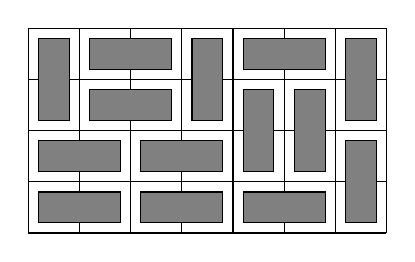
\begin{tikzpicture}[scale=.65]
    \draw (0,0) grid (7,4);
    \draw[fill=gray] (0+0.2,0+0.2) rectangle (2-0.2,1-0.2);
    \draw[fill=gray] (2+0.2,0+0.2) rectangle (4-0.2,1-0.2);
    \draw[fill=gray] (4+0.2,0+0.2) rectangle (6-0.2,1-0.2);
    \draw[fill=gray] (0+0.2,1+0.2) rectangle (2-0.2,2-0.2);
    \draw[fill=gray] (2+0.2,1+0.2) rectangle (4-0.2,2-0.2);
    \draw[fill=gray] (1+0.2,2+0.2) rectangle (3-0.2,3-0.2);
    \draw[fill=gray] (1+0.2,3+0.2) rectangle (3-0.2,4-0.2);
    \draw[fill=gray] (4+0.2,3+0.2) rectangle (6-0.2,4-0.2);

    \draw[fill=gray] (0+0.2,2+0.2) rectangle (1-0.2,4-0.2);
    \draw[fill=gray] (3+0.2,2+0.2) rectangle (4-0.2,4-0.2);
    \draw[fill=gray] (6+0.2,2+0.2) rectangle (7-0.2,4-0.2);
    \draw[fill=gray] (4+0.2,1+0.2) rectangle (5-0.2,3-0.2);
    \draw[fill=gray] (5+0.2,1+0.2) rectangle (6-0.2,3-0.2);
    \draw[fill=gray] (6+0.2,0+0.2) rectangle (7-0.2,2-0.2);

\end{tikzpicture}
\end{center}
ja ratkaisujen kokonaismäärä on 781.

Tehtävän voi ratkaista dynaamisella ohjelmoinnilla
käymällä ruudukkoa läpi rivi riviltä.
Jokainen ratkaisun rivi pelkistyy merkkijonoksi,
jossa on $m$ merkkiä joukosta $\{\sqcap, \sqcup, \sqsubset, \sqsupset \}$.
Esimerkiksi yllä olevassa ratkaisussa on 4 riviä,
jotka vastaavat merkkijonoja
\begin{itemize}
\item
$\sqcap \sqsubset \sqsupset \sqcap \sqsubset \sqsupset \sqcap$,
\item
$\sqcup \sqsubset \sqsupset \sqcup \sqcap \sqcap \sqcup$,
\item
$\sqsubset \sqsupset \sqsubset \sqsupset \sqcup \sqcup \sqcap$ ja
\item
$\sqsubset \sqsupset \sqsubset \sqsupset \sqsubset \sqsupset \sqcup$.
\end{itemize}

Tehtävään sopiva rekursiivinen funktio on $f(k,x)$,
joka laskee, montako tapaa on muodostaa ratkaisu
ruudukon riveille $1 \ldots k$ niin,
että riviä $k$ vastaa merkkijono $x$.
Dynaaminen ohjelmointi on mahdollista,
koska jokaisen rivin sisältöä
rajoittaa vain edellisen rivin sisältö.

Riveistä muodostuva ratkaisu on kelvollinen,
jos rivillä 1 ei ole merkkiä $\sqcup$,
rivillä $n$ ei ole merkkiä $\sqcap$
ja kaikki peräkkäiset rivit ovat \emph{yhteensopivat}.
Esimerkiksi rivit
$\sqcup \sqsubset \sqsupset \sqcup \sqcap \sqcap \sqcup$ ja
$\sqsubset \sqsupset \sqsubset \sqsupset \sqcup \sqcup \sqcap$ 
ovat yhteensopivat,
kun taas rivit
$\sqcap \sqsubset \sqsupset \sqcap \sqsubset \sqsupset \sqcap$ ja
$\sqsubset \sqsupset \sqsubset \sqsupset \sqsubset \sqsupset \sqcup$
eivät ole yhteensopivat.

Koska rivillä on $m$ merkkiä ja jokaiselle merkille on 4
vaihtoehtoa, erilaisia rivejä on korkeintaan $4^m$.
Niinpä ratkaisun aikavaativuus on $O(n 4^{2m})$,
koska joka rivillä käydään läpi $O(4^m)$
vaihtoehtoa rivin sisällölle
ja jokaista vaihtoehtoa kohden on $O(4^m)$
vaihtoehtoa edellisen rivin sisällölle.
Käytännössä ruudukko kannattaa kääntää niin
päin, että pienempi sivun pituus on $m$:n roolissa,
koska $m$:n suuruus on ratkaiseva ajankäytön kannalta.

Ratkaisua on mahdollista tehostaa parantamalla rivien esitystapaa merkkijonoina.
Osoittautuu, että ainoa seuraavalla rivillä tarvittava tieto on,
missä kohdissa riviltä lähtee laattoja alaspäin.
Niinpä rivin voikin tallentaa käyttämällä vain merkkejä
$\sqcap$ ja $\Box$, missä $\Box$ kokoaa yhteen vanhat merkit
$\sqcup$, $\sqsubset$ ja $\sqsupset$.
Tällöin erilaisia rivejä on vain $2^m$
ja aikavaativuudeksi tulee $O(n 2^{2m})$.

Mainittakoon lopuksi, että laatoitusten määrän laskemiseen
on myös yllättävä suora kaava
\[ \prod_{a=1}^{\lceil n/2 \rceil} \prod_{b=1}^{\lceil m/2 \rceil} 4 \cdot (\cos^2 \frac{\pi a}{n + 1} + \cos^2 \frac{\pi b}{m+1}).\]
Tämä kaava on sinänsä hyvin tehokas,
koska se laskee laatoitusten määrän ajassa $O(nm)$,
mutta käytännön ongelma kaavan käyttämisessä
on, kuinka tallentaa välitulokset riittävän tarkkoina lukuina.


